\chapter{相关基础研究}
\label{chapter:background}

本章将介绍普通和加密后重复数据删除、可信计算(TEE)等本文利用的基础知识,以及加密后重复数据删除系统中存在的性能瓶颈和安全性隐患。

\section{重复数据删除}
\label{sec:background-deduplication}

本文专注于基于数据块的重复数据删除,它以称为数据块的小型数据单元为粒度运行。基于数据块的重复数据删除比基于文件的重复数据删除更精细,因此通常具有更高的存储效率(节省更多的存储空间)。

基于数据块的重复数据删除有以下两种基本的数据块分块方法:

\begin{itemize}
    \item \textbf{固定大小的数据分块(Fixed-size chunking)},通常将文件划分为固定长度的数据块,具有简单快速的特点,但文件中小范围修改(例如:增加1字节内容或删除1字节内容)将从修改位置开始影响后续所有数据块的内容,不利于重复数据删除。
    \item \textbf{可变大小的数据分块(Variable-size chunking)},也称为内容定义的数据块分块(Content-defined chunking)。通常采用内容相关的方式指定数据块的边界(例如,通过Rabin指纹\cite{rabin1981fingerprinting}在特定内容模式出现时进行分块)。因此,在文件发生小范围修改时,产生的大多数数据块仍可保持不变,使得重复数据删除系统存储效率得到保障。
\end{itemize}

在多数备份系统工作负载\cite{zhu2008avoiding,lillibridge2009sparse}下,可变大小的数据分块方案通常可以获得更优的存储效率,但在某些特定工作负载(例如,VM备份数据集\cite{jin2009effectiveness})下,固定大小的数据分块方案却更加有效。本文的工作可兼容固定大小和可变大小的数据分块方法产生的数据块。

\begin{figure}[!htb]
    \small
    \centering
    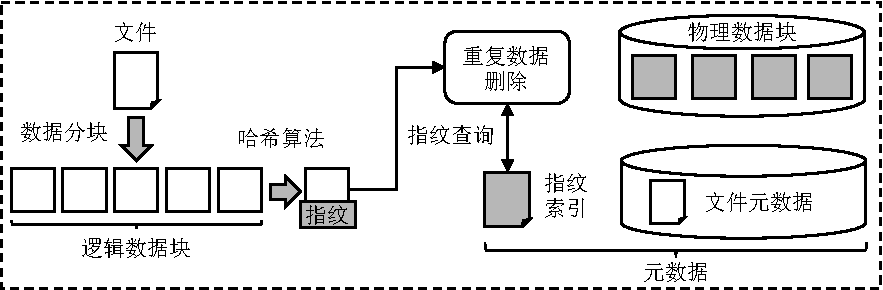
\includegraphics[width=\textwidth]{chunk-based-dedup-arch.pdf}
    \caption{基于数据块的重复数据删除的工作流程概览} 
    \label{fig:chunk-based-dedup-flow}
\end{figure}

图\ref{fig:chunk-based-dedup-flow}总结了基于数据块的重复数据删除工作流程。具体地,重复数据删除系统首先通过数据分块过程将客户端的文件(例如,备份文件)分割为逻辑数据块,根据每一个逻辑数据块的内容,使用哈希算法计算得到其对应的唯一标签(又称为指纹)。如果两个数据块具有相同的指纹,则认为两个数据块内容相同(不同逻辑数据块计算得到相同指纹的概率可忽略不计\cite{black2006compare});若两个逻辑数据块指纹不一致,则认为两逻辑数据块不同。重复数据删除系统仅存储相同逻辑数据块的唯一副本(称为物理数据块),并且每个相同的逻辑数据块仅通过一个空间开销较小的索引指向相同的物理数据块。此外,基于数据块的重复数据删除系统记录文件所拥有的所有逻辑数据块的信息作为该文件的元数据,用于文件读取、删除等操作。

重复数据删除技术根据重复数据删除操作发生的位置可分为源端重复数据删除及目标端重复数据删除\cite{IDC2010Data}:

\begin{itemize}
    \item \textbf{源端重复数据删除(Source-based Deduplication)}由客户端计算目标数据块的哈希值,并由服务端检查该哈希值是否存在于索引表中。如果哈希值存在(即服务端已有目标数据块的副本),则通知客户端无需传输目标数据块。
    \item \textbf{目标端重复数据删除(Target-based Deduplication)}强制客户端传输所有密文数据块,并在服务端对所有收到的密文数据块进行重复数据删除。
\end{itemize}

源端重复数据删除技术可有效节省网络流量资源,可显著降低云服务商提供存储服务的成本,但泄露了“其他客户端是否已经存储相应密文数据块”的侧信道信息(参见\S\ref{subsubsec:intro-problem-security});目标端重复数据删除具有更高的隐私保护能力,但产生大量网络资源浪费,并显著增加了服务端计算开销。本文关注网络资源开销较小的源端重复数据删除技术,并通过TEE技术解决其存在的性能和安全性问题。

\section{安全重复数据删除}
\label{sec:background-enc-deduplication}

加密后重复数据删除解决了外包环境(例如,云存储)中的数据块机密性保障问题,同时保持了重复数据删除的有效性。出于安全因素考虑,用户希望将自己的数据加密后再进行外包存储,以确保个人数据隐私性。传统对称加密算法算法为每个客户端或每个逻辑数据块分配独立的加密密钥,使得来自不同(或相同)客户端的相同的逻辑数据块被加密为不同的密文数据块,服务器无法感知这些密文数据块所对应的明文数据块内容是否一致,使得针对外包数据的重复数据删除完全失效。

\begin{figure}[!htb]
    \small
    \centering
    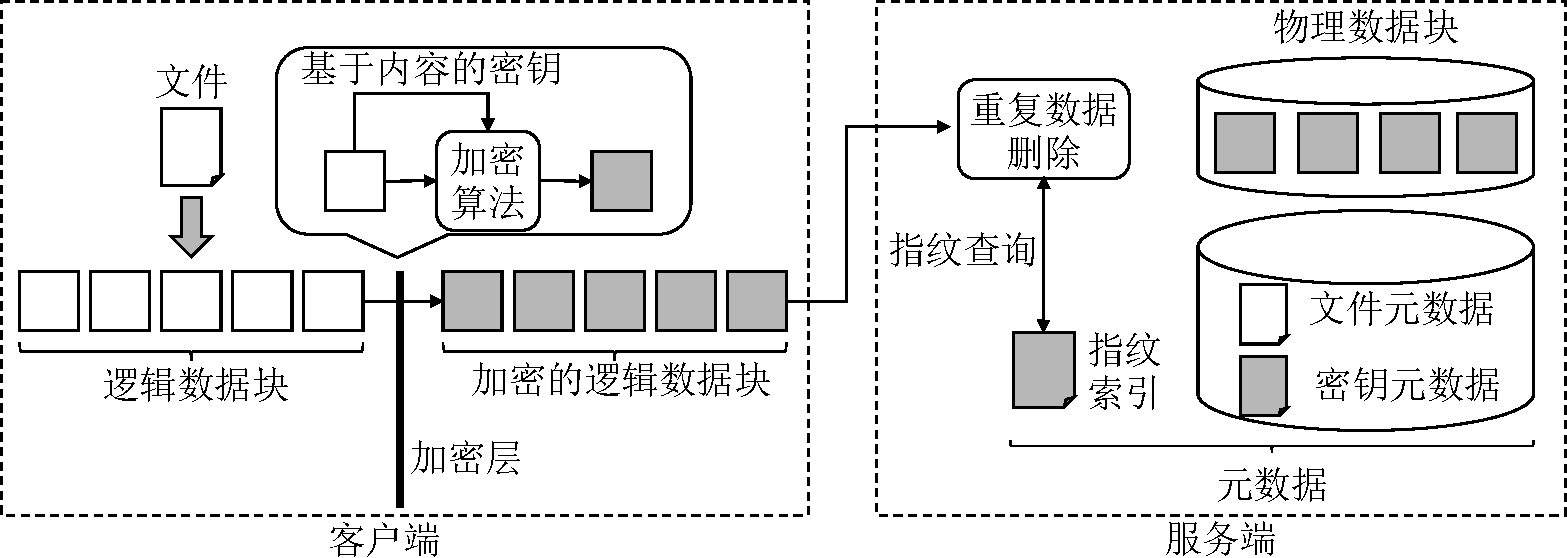
\includegraphics[width=\textwidth]{chunk-based-enc-dedup-arch.pdf}
    \caption{基于数据块的加密后重复数据删除的工作流程概览} 
    \label{fig:chunk-based-enc-dedup-flow}
\end{figure}

如图~\ref{fig:chunk-based-enc-dedup-flow}所示,基于内容的密钥生成方法给加密后重复数据删除提供了新的处理思路。最基本的基于内容的密钥生成方法的实例化是基于明文数据的内容(例如,基于重复数据删除中的逻辑数据块)导出其对称加密密钥,并使用该密钥加密明文数据以形成对应的密文数据(例如,加密的逻辑数据块)。因此,使用基于内容的密钥生成方法为任意逻辑数据块产生对称加密密钥可以确保将相同的明文数据块加密为相同的密文数据块。最后,存储系统从每个密文数据块中导出其对应的指纹并执行重复数据删除。相较于普通重复数据删除,加密后重复数据删除需额外保存用户文件所包含数据块的密钥元数据,并由各个客户端进行加密以防止服务端取得相应数据块的明文内容。

\subsection{数据块加密技术}
\label{subsec:background-encrypted-deduplication-key}

\textit{消息锁加密(Message-Locked Encryption, MLE)}\cite{bellare2013MLE}将基于内容的密钥生成方案等加密原语形式化用于加密后重复数据删除。它指出了如何从明文数据块的内容导出相应的对称加密密钥(称为 \textit{消息锁加密密钥(MLE密钥)})。以最广泛使用的消息锁加密技术:收敛加密(Convergent Encryption, CE)\cite{douceur2002reclaiming}为例,CE使用明文数据块的安全哈希作为MLE密钥,使得相同的明文数据块可被加密为相同的密文数据块,从而令重复数据删除技术在密文数据块之上仍然可行。除此之外,基于CE的消息锁加密方案还包括:

\begin{enumerate}
    \item \textbf{哈希收敛加密(Hash Convergent Encryption, HCE)}\cite{douceur2002reclaiming}与CE具有相同的MLE密钥产生规则,但基于明文哈希值计算指纹用于重复数据删除(CE使用密文指纹进行重复数据删除)。
    \item \textbf{随机收敛加密(Random Convergent Encryption, RCE)}\cite{douceur2002reclaiming}使用随机密钥加密明文以产生非确定的密文,但基于明文的哈希值进行重复数据删除检查。
    \item \textbf{收敛扩散(Convergent Dispersa, CD)}\cite{li2016cdstore}使用明文哈希值作为秘密共享(Secret Sharing)的输入种子,并对产生的多个秘密共享分别计算哈希并进行重复数据删除,在兼容重复数据删除的基础上提高了密文存储的可靠性。
\end{enumerate}

然而,CE容易受到\textbf{离线暴力破解攻击}的威胁。这是由于CE的MLE密钥(即明文数据块的哈希)可以自由产生。具体来说,攻击者通过枚举所有可能的明文数据块的MLE密钥来从目标密文数据块(其加密密钥未知)推断输入的明文数据块,以检查是存在某个明文数据块被加密到目标密文数据块。

服务器辅助消息锁加密(Server-aided MLE)\cite{bellare2013DupLESS}是最先进的加密原语,可增强加密后重复数据删除对离线暴力攻击的安全性。它为消息锁加密中的MLE密钥生成步骤部署了一个专用的\textbf{密钥服务器(key server)}。为了加密明文数据块,客户端首先将明文数据块的指纹发送到密钥服务器,密钥服务器通过指纹和密钥服务器维护的\textbf{全局秘密(global secret)}返回MLE密钥。如果全局秘密是安全的,则攻击者无法发起离线暴力攻击;如果全局秘密被泄露,则其安全性会降低到原始消息锁加密的安全性。服务器辅助消息锁加密建立在如下两种安全机制之上:

\begin{itemize}
    \item \textbf{遗忘伪随机函数(oblivious pseudorandom function, OPRF)}\cite{naor2004Number}是一种安全计算协议,协议包含服务端和客户端,服务端持有密钥$k$,客户端持有输入$x$,双方通过交互来联合计算函数$f_k(x)$,最终由客户端得到函数值。OPRF的计算过程以盲化方式进行,即在计算过程中服务端无法获取关于$x$的任何有价值信息,同时客户端无法获取关于$k$的任何有价值信息。
    \item \textbf{速率限制(Rate-limiting)}\cite{bellare2013DupLESS}阻止特定操作频率超出某些限制。在大型系统中,速率限制通常用于保护底层服务和资源。
\end{itemize}

基于遗忘为随机函数,密钥服务器可依据客户端发送明文数据块的“盲指纹”,进而基于盲指纹和全局秘密产生对应数据块的“盲密钥”,阻止了密钥服务器了解明文数据块信息;并使得客户端可在不了解密钥服务器所拥有的全局秘密的条件下获得目标明文数据块的MLE密钥。对来自客户端的密钥生成请求进行速率限制,进一步防止恶意客户端向密钥服务器发出海量密钥生成请求以获得目标MLE密钥,限制了攻击者暴力破解攻击的速度。

\subsection{数据所有权证明}
\label{subsec:background-encrypted-deduplication-pow}

为了节省宝贵的网络带宽资源,现有加密后重复数据删除系统普遍采用源端重复数据删除,以便在客户端删除重复数据块,而无需上传到服务端(\S\ref{sec:background-deduplication})。但是,当某些客户端存在恶意时,源端重复数据删除很容易受到侧信道攻击(\textit{Side-channel Attack})\cite{harnik2010side,halevi11}。一种典型侧信道攻击是,恶意客户端将目标密文数据块指纹发送到服务端以检查该数据块是否存在(例如,目标密文数据块对应于某个可能的密码\cite{harnik2010side}),以此识别来自其他客户端的敏感信息(\S\ref{subsubsec:intro-problem-security});另一种侧信道攻击是,恶意客户端未授权访问其他客户端存储的数据块(\S\ref{subsec:intro-background})。具体来说,由于服务端仅能基于收到的数据块哈希值判断客户端是否拥有对应的数据块,攻击者可使用任意目标密文数据块的指纹来说服服务端其是该目标数据块的所有者,进而获得该数据块的完全访问权限\cite{halevi11}。

另一方面,重复数据删除受到伪造数据所有权的攻击威胁\cite{harnik2010side,mulazzani11}。由于云服务商仅基于收到的数据块哈希值判断客户端是否拥有相应数据块,恶意用户/客户端可以伪造任意密文数据块的哈希值,如果该密文数据块已在云端存储(即已发生重复数据删除),则恶意客户端无需传输密文数据块内容便可获得相应密文数据块的访问权限。为了防止伪造所有权攻击,加密后重复数据删除增加了所有权证明(proof-of-ownership)技术\cite{halevi11}:除了密文数据块的哈希值以外,云服务商要求客户端额外提交目标密文数据块的所有权证明(proof);云服务商首先基于证明验证该客户端是否真实且完整拥有相应密文数据块,然后再执行如前所述的重复数据删除过程。所有权证明技术的合理性在于,只针对客户端真实拥有(即具有完整访问权限)的密文数据块执行重复数据删除,从而避免非法访问其他客户端已在云端存储的内容。

%TODO
\textbf{所有权证明(Proof-of-Ownership, PoW)}\cite{halevi11}是一种密码学机制,可增强源端重复数据删除,防止侧信道攻击,同时保持源端重复数据删除的网络资源节省。

它的想法是让云验证客户端确实是密文数据块的所有者,并被授权完全访问密文数据块。这确保了受感染的客户端无法查询其他客户端的块是否存在。

具体来说,在基于 PoW 的源端重复数据删除中,客户端将发送到云的每个指纹都附加一个\textit{ PoW 证明},云可以通过它验证客户端是否是相应密文数据块的真正所有者。云仅对成功的证明验证做出响应,从而防止任何受感染的客户端识别其他客户端拥有的密文数据块。 


% 基于Merkel树(Merkel Tree)的所有权证明(POW-MT),该方案使用纠删码对数据块进行编码,在编码结果基础上建立Merkel树用于所有权证明,具体证明过程可参考文献《J. Xu, E.-C. Chang, and J. Zhou. Weak leakage-resilient client-side deduplication of encrypted data in cloud storage. In Proc. of ACM ASIACCS, 2013》。
% 2)基于通用哈希函数的所有权证明(PoW-UH),它建立在通用散列的基础上,但为了性能而牺牲了安全性,具体证明过程可参考文献《S. Halevi, D. Harnik, B. Pinkas, and A. Shulman-Peleg. Proofs of ownership in remote storage systems. In Proc. of ACM CCS, 2011]》。

本文着眼于基于TEE实现高效的服务器辅助消息锁加密以及数据块所有权证明机制,

数据所有权证明


关注网络资源开销较小的源端重复数据删除技术,并通过TEE技术解决其存在的性能和安全性问题。


\section{可信执行环境(TEE)}
\label{sec:background-tee}

TEE全名为可信执行环境(Trusted Execution Environment)是计算平台上由软件协同硬件方法构建的一个安全区域,可以确保在安全区域内加载的程序和数据在完整性和机密性方面得到必要保护。其目标是确保目标程序按照预期执行,保证程序初始状态和运行时状态的机密性、完整性。针对TEE的相关概念及规范定义,各个软件、硬件厂商结合自己的基础架构形态产生的具体实现各不相同。虽然在技术实现上存在显著差异,但TEE的技术共同点可总结为如下三点:

\begin{itemize}
    \item \textbf{隔离性}:
    TEE通过隔离的程序执行环境,提供一个可信的执行空间,为其中运行的程序和存储的数据提供了机密性和完整性保护。X86架构的隔离机制从Intel 80286处理器开始,Intel提出了CPU的两种运行模式,并且逐步衍生出后来的不同的特权界别,再后来提出了安全区域范围更小的SGX机制实现可信执行环境TEE;同样的,ARM架构通过TrustZone技术实现了相关软硬件的隔离性,实现了安全世界(Secure World)与非安全世界(Normal World)的隔离。
    \item \textbf{软硬协同性}:
    虽然标准定义可以通过单独软件方式或单独硬件方式实现TEE,但实际应用场景下,行业内更多选择通过软硬件结合的方式进行TEE的设计。
    \item \textbf{富表达性}:
    与传统安全新芯片或纯软件的密码学营私保护方案相比,TEE支持的上层业务表达性更强,软件开发者仅需要根据业务逻辑划分业务层面的隐私和非隐私区域,而不会对定义隐私区域内的算法逻辑的语言等有可计算性方面的限制(图灵完备的)。同时,由于TEE为程序提供了可信的执行环境,安全区内的数据无需进行密态运算,使得TEE应用可以支持更多的算计及复杂的算法。
\end{itemize}

\subsection{Intel SGX}
\label{subsec:background-tee-sgx}

\begin{figure}[!htb]
    \small
    \centering
    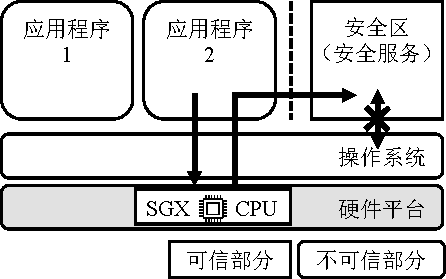
\includegraphics[width=0.6\textwidth]{sgx-example.pdf}
    \caption{Intel SGX框架} 
    \label{fig:sgx-arch}
\end{figure}



Intel® Software Guard Extensions(英特尔® SGX)是一组用于增强应用程序代码和数据安全性的指令,开发者使用SGX技术可以把应用程序的安全操作封装在一个被称之为Enclave的容器内,保障用户关键代码和数据的机密性和完整性。

Intel Software Guard Extensions (Intel SGX)\cite{sgx,sgx2},是一组内置于现代Intel CPU中用于增强应用程序代码和数据安全性的扩展指令。开发者可利用SGX技术将应用程序的安全操作封装在称为“安全区(Enclave)”的硬件保护环境中。Intel SGX具有隔离、证明和密封三项主要安全功能(ru'xii'iiiiiiiiiiiiiiiiiiiiiiiiiiiiiiiiiiiiiiiiiiiiii),可为。

\paragraph*{Isolation.}安全区驻留在称为\textit{安全区page cache (EPC)} 的硬件保护内存区域中,用于托管任何受保护的代码和数据。一个 EPC 包含 4KB 页面,任何 in-enclave 应用程序最多可占用 96\,MB \cite{harnik18}。如果安全区的大小比 EPC 大,它会加密未使用的页面并将它们驱逐到未受保护的内存中。在这项工作中,本文在每个客户端和密钥服务器中部署安全区以保护敏感操作 (\S\ref{subsec:sgxdedup-arch})。本文还限制了 in-enclave 内容的大小以减轻分页开销 (\S\ref{subsec:sgxdedup-encryption})。

enclave 提供了一个接口,即 \textit{安全区call (ECall)},以便外部应用程序可以发出 ECall 以安全地访问安全区内的内容。请注意,ECall 会产生访问安全区内存 \cite{harnik18} 的上下文切换开销。本文通过批量处理内容来减少 ECall 的数量(\S\ref{sec:sgxdedup-implementation})。

\paragraph*{Attestation.} SGX 支持 \textit{ 远程认证} 通过远程实体(例如云)对目标安全区进行身份验证。在远程证明过程中(详见\cite{sgx}),远程实体需要联系Intel运营的证明服务来检查目标enclave提供的enclave信息的完整性。然后,远程实体通过将其安全区信息与目标安全区中预期的可信配置进行比较来验证目标 enclave。本文使用远程证明来确保在第一个引导程序中将正确的代码和数据加载到每个安全区中。

\paragraph*{Sealing.} SGX 通过密封将安全区内容存储在安全区外部时对其进行保护。它使用秘密 \textit{ 密封密钥} 在被驱逐之前加密数据。密封密钥可以从 \textit{ 测量散列}(即安全区内容的 SHA256 散列)或安全区的作者身份派生,因此只有相应的安全区才能访问密封密钥并解密密封数据.由于远程证明会导致显着延迟(Exp\#7),本文使用密封来消除安全区第一次引导后的远程证明(\S\ref{subsec:sgxdedup-enclave-management})。

\subsection{ARM TrustZone}
\label{subsec:background-tee-tz}

与TEE相对应的fu'zhi'xing REE(Rich Execution Environment)概念,分别对应于安全世界(Secure World)和非安全世界(Non-secure World, Normal World)。


\subsubsection{TrustZone}


ARM TrustZone是ARM公司针对消费电子设备设计的一种TEE解决方案,其目的是为消费电子产品构建一个安全框架来抵御各种可能的攻击,它通过对原有硬件架构进行修改,在处理器层次引入了两个不同权限的保护域:安全世界和非安全世界,任何时刻处理器仅在其中的一个环境内运行。

同时这两个世界完全是硬件隔离的,并具有不同的权限,正常世界中运行的应用程序或操作系统访问安全世界的资源受到严格的限制,反过来安全世界中运行的程序可以正常访问正常世界中的资源。

各芯片产商会根据ARM公司对于TrustZone的硬件设计在具体的芯片上进行设计和实现,基于TrustZone技术,可以搭建一个可信执行环境TEE,在TEE内可以有基于TrustZone的操作系统,如高通的QSEE、开源的OPTEE等


TrustZone是ARM

TrustZone在概念上将SoC的硬件和软件资源划分为安全(Secure World)和非安全(Normal World)两个世界,所有需要保密的操作在安全世界执行(如指纹识别、密码处理、数据加解密、安全认证等),其余操作在非安全世界执行(如用户操作系统、各种应用程序等),安全世界和非安全世界通过一个名为Monitor Mode的模式进行转换,如图1:

处理器架构上,TrustZone将每个物理核虚拟为两个核,一个非安全核(Non-secure Core, NS Core),运行非安全世界的代码;和另一个安全核(Secure Core),运行安全世界的代码。

两个虚拟的核以基于时间片的方式运行,根据需要实时占用物理核,并通过Monitor Mode在安全世界和非安全世界之间切换,类似同一CPU下的多应用程序环境,不同的是多应用程序环境下操作系统实现的是进程间切换,而Trustzone下的Monitor Mode实现了同一CPU上两个操作系统间的切换。


图中左边蓝色部分Rich OS Application Environment(REE)表示用户操作环境,可以运行各种应用,例如电视或手机的用户操作系统,图中右边绿色部分Trusted Execution Envrionment(TEE)表示系统的安全环境,运行Trusted OS,在此基础上执行可信任应用,包括身份验证、授权管理、DRM认证等,这部分隐藏在用户界面背后,独立于用户操作环境,为用户操作环境提供安全服务。



TrustZone是ARM A/M系列处理器中的安全架构扩展。其随ARM v6K指令集发布,并在之后的ARM v7,v8,以及正在开发中的v9指令集中得到支持。TrustZone 提供了两个相互独立的指令执行环境,它们之间具有涵盖系统范围的硬件强制隔离,如下图~\ref{fig:ARM-TZ-base}所示:

\begin{figure}[!htb]
    \small
    \centering
    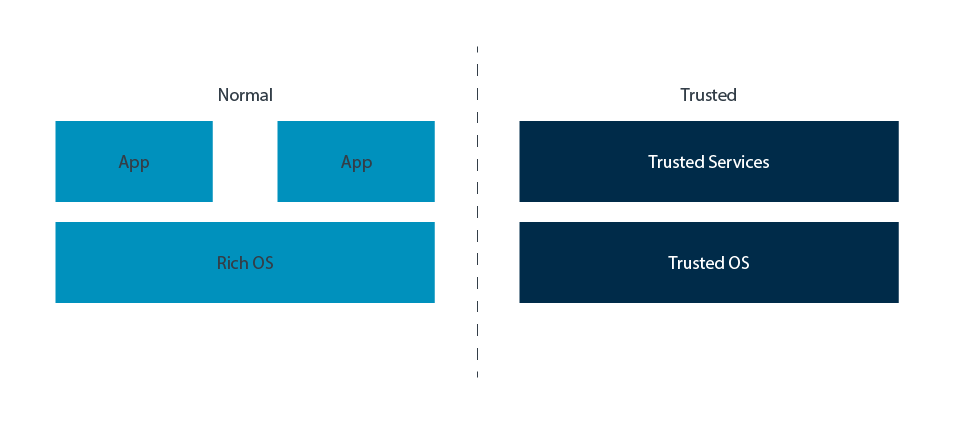
\includegraphics[width=\textwidth]{ARM-TZ-base.png}
    \caption{ARM TrustZone结构示意图} 
    \label{fig:ARM-TZ-base}
\end{figure}

非安全世界(Normal)运行着规模庞大的软件栈,称为。其软件栈通常包括多个应用程序集、一个复杂的操作系统(如 Linux)以及可能的管理程序。此类软件堆栈庞大而复杂。虽然可以努力保护它们,但攻击面的大小意味着它们更容易受到攻击。

而与非安全世界对应的可信世界运行着一个更精简的软件栈,称为可信执行环境 (TEE)。通常,TEE 包括由轻量级内核托管的多个可信服务。受信任的服务提供密钥管理等功能。该软件堆栈的攻击面要小得多,这有助于减少易受攻击的脆弱性。

注意:您有时可能会看到术语富执行环境 (REE) 用于描述在正常世界中运行的软件。

TrustZone 旨在形成一个圆形。作为用户和开发人员,我们想要 Normal 世界的丰富功能集和灵活性。同时,我们希望在受信任的世界中使用更小、更受限制的软件堆栈来实现更高程度的信任。 TrustZone 为我们提供了两者,提供了两个环境,它们之间具有硬件强制隔离。

\subsubsection{OP-TEE}

OP-TEE 是一种可信执行环境 (TEE),旨在与在 Arm 上运行的非安全 Linux 内核配套使用; 使用 TrustZone 技术的 Cortex-A 内核。 OP-TEE 实现了 TEE 内部核心 API v1.1.x,它是公开给可信应用程序的 API 和 TEE 客户端 API v1.0,它是描述如何与 TEE 通信的 API。 这些 API 在 GlobalPlatform API 规范中定义。

\begin{figure}[!htb]
    \small
    \centering
    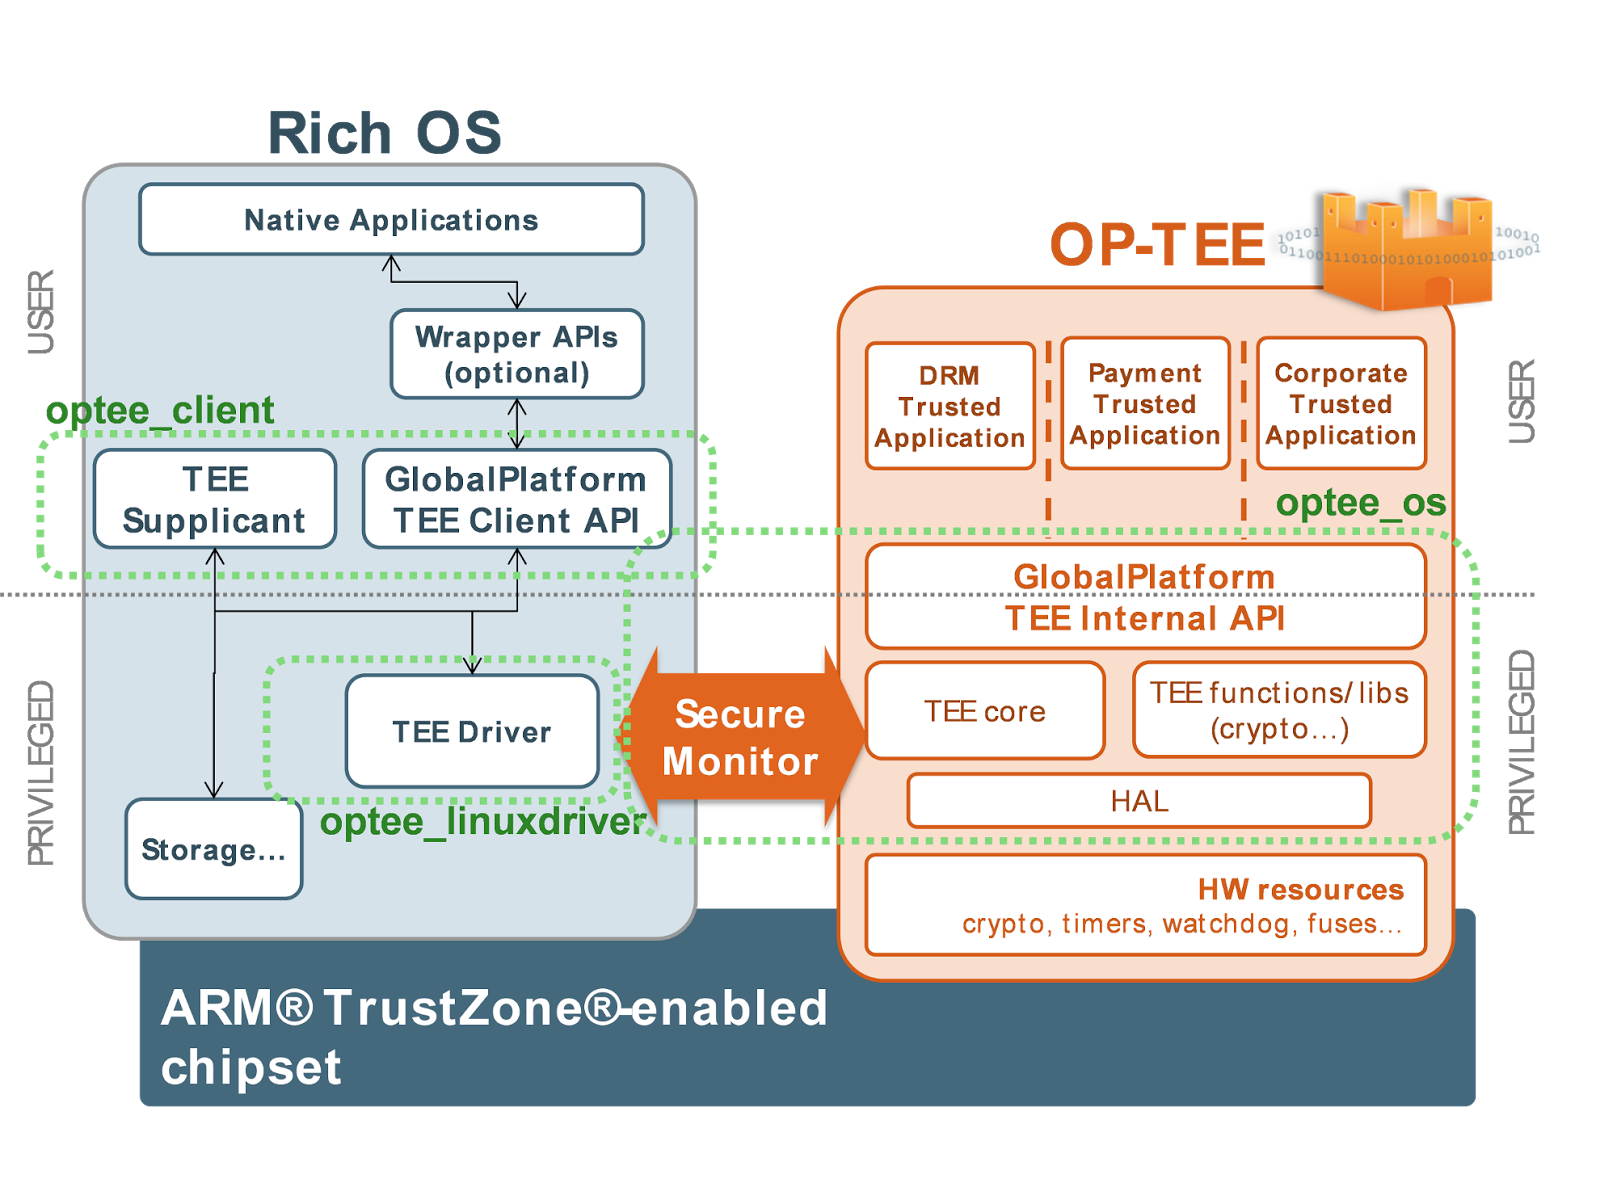
\includegraphics[width=\textwidth]{OP-TEE.png}
    \caption{OP-TEE的架构设计} 
    \label{fig:ARM-TZ-CPU}
\end{figure}

非安全操作系统在 TEE 规范中称为富执行环境 (REE)。 它通常是作为 GNU/Linux 发行版或 AOSP 的 Linux 操作系统风格。OP-TEE 的设计主要依赖于 Arm TrustZone 技术作为底层硬件隔离机制。 但是,它的结构与任何适合 TEE 概念和目标的隔离技术兼容,例如作为虚拟机运行或在专用 CPU 上运行。

OP-TEE 的主要设计目标是:
\begin{itemize}
    \item 隔离 - TEE 提供与非安全操作系统的隔离,并使用底层硬件支持保护加载的可信应用程序 (TA),
    \item 占用空间小 - TEE 应保持足够小,以驻留在基于 Arm 的系统上的合理数量的片上内存中,
    \item 可移植性 - TEE 旨在轻松插入不同的架构和可用的硬件,并且必须支持各种设置,例如多个客户端操作系统或多个 TEE。
\end{itemize}

